% !TEX root = ../thesis.tex

\chapter{Markov跳变Lur'e系统的异步控制及$\ell_2$性能分析}
	非线性是控制系统中普遍存在的现象之一。由于非线性的存在可能会严重影响控制系统的工作状态,甚至破坏系统的稳定性,所以研究非线性系统具有重要的意义,得到了众多学者的关注。上个世纪四十年代,前苏联数学家Lur'e在研究飞行器驾驶技术时,发现了一种用有限或者无线扇形区间约束的非线性,自此Lur'e系统\cite{lurie1957some}进入了人们的视野。一般来说,完整的Lur'e由一个线性环节和一个满足有限、无限扇形区间的非线性环节串联组成\cite{khalil2002nonlinear},如
	\begin{equation}
		\left\{
			\begin{array}{lr}
			x_{k+1}=Ax_k+Bf(y_k),\\
			y_k=Cx_k.
			\end{array}
		\right.
	\end{equation}
	Lur'e系统凭借其普遍存在性、广泛适用性,获得了广大学者们的关注。学者们对其进行了深入的研究并取得了一系列重要的成果\cite{kalman1963lyapunov,park2002stability,suykens1997nonlinear,cao2005synchronization}。特别的,在文献\cite{castelan2006absolute,castelan2008control}中,作者针对分别对连续、离散域Lur'e系统的绝对稳定性问题,并在文中提出了一种新型反馈控制结构,该结构由一个线性状态反馈和非线性输出反馈组成,且该非线性是同Lur'e系统中的非线性是保持一致的。这种结构相对于一般的线性状态反馈控制器会更加的灵活,并且会降低得到结果的保守性。文献\cite{gonzaga2012stability}对离散Markov跳变Lur'e系统的稳定性进行了研究,并提出了一种Lur'e型李雅普诺夫函数来研究Lur'e系统,进一步降低了得到结果的保守性。同时,Lur'e系统的研究并没有局限在理论层面,随着研究深入,在诸如机器人控制\cite{mahmoud1994globally,chen1999controlling},飞行器\cite{leonov2012aircraft},网络通信\cite{li2006stability}等领域中。
	
	Markov跳变Lur'e系统在近年来也取得了一系列重要的理论成果。文献\cite{zhu2015distributed,zhang2017resilient,zhang2015model}分别对Markov跳变系统的$H_\infty$滤波、无源控制、模型推导问题进行了研究。文章\cite{gonzaga2014stochastic,song2012stability}对一类控制器饱和非线性的Markov跳变控制系统的稳定性和$l_2$性能进行了研究。文章\cite{wu2012stochastic}对一类具有时变时滞和分段恒定转移概率的奇异Markov跳变Lur'e系统进行了讨论。值得注意的是,上述结果基本上都基于控制器模态同系统模态完全匹配这一完美假设。而对模态不匹配的Markov跳变Lur'e系统的研究成果比较少。在文章\cite{song2018event}中,作者结合了事件触发和隐Markov模型,探究了Markov跳变系统的滑模控制问题。
	
	本章中,考虑到控制器模态同系统模态不一致的问题,我们将引入隐Markov模型,来研究一类Markov跳变Lur'e系统的异步控制问题,并对系统的稳定性及$l_2$性能进行讨论。

\section{数学模型及问题描述}
	本章考虑下面的Markov跳变Lur'e系统:
	\begin{equation}\label{syseq}\left\{
	\begin{array}{lr}
		\begin{split}
			x_{k+1}=A_{r(k)}x_k+F_{r(k)}\varphi(y_k)+B_{r(k)}u_k +E^x_{r(k)}w_,
		\end{split}\\
		\begin{split}
			y_k=C_{r(k)}x_k,
		\end{split}
		\\
		\begin{split}
			z_k= C^z_{r(k)}x_k+G^z_{r(k)}\varphi(y_k)+D^z_{r(k)}u_k+E^z_{r(k)}w_k,
		\end{split}	
	\end{array}\right.
	\end{equation}
	其中,$x_k\in\mathbb{R}^{n_x}$ 表示系统状态, $u_k\in\mathbb{R}^{n_u}$ 表示控制输入, $y_k\in\mathbb{R}^{n_y}$ 表示一个包含非线性的观测输出,$ z_k\in\mathbb{R}^{n_z}$ 表示被控输出, $w_k\in\mathbb{R}^{n_w}$ 表示外界扰动。 $A_{r(k)}$, $F_{r(k)}$, $B_{r(k)}$, $E^x_{r(k)}$, $C^z_{r(k)}$,$G^z_{r(k)}$, $D^z_{r(k)}$ 及 $E^z_{r(k)}$ 是已知的实系统矩阵且具备合适维度。
	$\{r(k),k\geq0\}$ 是一个Markov链,且在集合 $\mathcal{N}=\{1,2,\dots,N\}$ 中取值,并且满足如下模态转移概率:
	\begin{equation}
	\Pr\{r(k+1)=j|r(k)=i\}=\pi_{ij},
	\end{equation}
	其中,$\pi_{ij}\in[0,1]$, 对任意的 $i,j\in\mathcal{N}$,且 $\sum_{j=1}^{N}\pi_{ij}=1$ 对任意的模态 $i$. 在 $i$ 时刻的系统矩阵可以记作 $A_i$,$F_i$,$B_i$,$E^x_i$,$C^z_i$,$G^z_i$,$D^z_i$,且相应的模态转移矩阵可以表示为 $\varPi=\{\pi_{ij}\}$.
	
	首先,我们对非线性 $\varphi(\cdot)$ 做如下的假设
	
	{\bf 定义 \ \ 2.1:} 
	非线性 $\varphi(\cdot): \mathbb{R}^{n_y}\rightarrow\mathbb{R}^{n_y}$ 满足一个有界扇形条件,如果下面两个条件能够同时满足:
		
		(1) $\varphi(0)=0$ 
		
		(2) 存在正定矩阵 $\varOmega \in\mathbb{R}^{n_y\times n_y}$,对任意的 $y\in\mathbb{R}^{n_y}$, $\nu \in\{1,\dots,n_y\}$,使得下式成立 
		\begin{equation}\label{cbs} 
		\varphi_{(\nu)}(y)[\varphi(y)-\varOmega y ]_{(\nu)}\leq 0
		\end{equation}
		
	由 \eqref{cbs}式,我们可以推出
	\begin{equation}\label{scieq}
	SC(y,\varLambda):= \varphi^{\mathrm{T}}(y)\varLambda[\varphi(y)-\varOmega y]\leq0,
	\end{equation}
	其中,$\varLambda$ 是任意的半正定矩阵, 且 $\varOmega$ 可以由设计者自己预先给出。然后我们根据上式可以进一步推出
	\begin{equation}
	[\varOmega y]_{(\nu)}[\varphi(y)-\varOmega y]_{(\nu)}\leq0,
	\end{equation}
	这个式子可以进一步得到
	\begin{equation}
	0\leq\varphi^{\mathrm{T}}(y)\varLambda\varphi(y) \leq \varphi^{\mathrm{T}}(y)\varLambda\varOmega y \leq y^{\mathrm{T}}\varOmega\varLambda\varOmega y
	\end{equation}
	
	下面我们给出系统稳定性的定义
	
	{\bf 定义 \ \ 2.1:} 
	当 $w(k)\equiv0$ 时,我们称系统 \eqref{syseq} 是随机稳定的,如果
	\begin{equation}
	\|x\|^2_2=\sum_{k=0}^{\infty}\mathbb{E}[\|x_k\|^2]<\infty.
	\end{equation} 
	
	下面我们给出系统 $\ell_2$ 性能定义
	
	{\bf 定义 \ \ 2.2:}
	给定一个正标量 $\zeta$, 定义如下集合 $\mathcal{W}_{\zeta} $ 	
	\begin{equation}
		\begin{split}
			\mathcal{W}_{\zeta}&:=\Big\{ w=\{w_k\}; \   \|w\|^2_2=\sum_{k=0}^{\infty}\mathbb{E}[\|w_k\|^{2}]<\zeta\Big\}\\
		\end{split}
	\end{equation}
	对任意的  $w\in\mathcal{W}_{\zeta}$, 如果下式成立
	\begin{equation}
		\|z\|^2_2=\sum_{k=0}^{\infty}\mathbb{E}\left[\|z_k\|^2\right] \leq \gamma^{2}\|w\|^2_2
	\end{equation}
	那么,我们称在零初始条件下,系统在外界扰动 $w=\{w_k\}$ 及控制输出 $z=\{z_k\}$ 间的 $\ell_2$ 增益是小于等于 $\gamma$ 的。
	
	在本章中,我们考虑如下异步控制器
	\begin{equation}\label{asycontroller}
	u_k=K_{\sigma(k)}x_k+\varGamma_{\sigma(k)}\varphi(y_k) 
	\end{equation}
	其中 $K_{\sigma(k)}\in \mathbb{R}^{n_u\times n_x}$ 是一个时变线性状态反馈矩阵, $\varGamma_{\sigma(k)}\in \mathbb{N}^{n_u\times n_y}$ 表示非线性时变输出反馈矩阵。 参数 $\sigma(k)$ 表示控制器的模态,且在集合  $\mathcal{M}=\{1,2,\dots,M\}$ 中取值,并且满足条件模态转移矩阵 $\varPhi=\{\mu_{i\phi} \}$,该矩阵对应的条件模态转移概率为
	\begin{equation}
	\Pr\{\sigma(k)=\phi|r(k)=i\}=\mu_{i\phi}
	\end{equation}
	其中,对任意的 $i\in\mathcal{N}$ 及 $\phi\in\mathcal{M}$ 有 $\mu_{i\phi}\in [0,1]$,且对任意的模态 $i$ 有 $\sum_{\phi=1}^{M}\mu_{i\phi}=1$。
	
	{\bf 注 \ \ 2.1:} 
	同 \cite{wu2016passivity} 相似,本章中采用了隐Markov模型来描述出现在系统与控制器之间的模态不匹配现象。不难发现,我们设计的控制器包含了一个线行的状态反馈部分,还包含了一个满足假设一的非线性输出反馈部分,这可以使得我们得到的结果更加的不保守。不同于之前同步控制器的设计方法,如\cite{song_control} 及 \cite{costaolv_control_1},本章中设计的控制器是一个异步控制器,这意味着系统模态和控制器模态在同一时刻可能是不同的。 显然,当条件模态转移矩阵 $\varPhi$ 是一个单位矩阵的时候,控制器模态会与系统模态保持一致,即,控制器会变成了一个同步控制器。 同时,如果控制器的模态只有一个的时候,我们可以认为此时系统是模态无关。也就是说,基于隐Markov模型的异步控制器设计方法,可以通过改变模态转移概率矩阵,使得异步控制器转变为同步控制器或者特殊的模态无关控制器。
	
	根据系统方程 \eqref{syseq} 和控制器 \eqref{asycontroller}, 我们可以得到如下闭环控制系统
	\begin{equation}\label{close_system_equation_2}
	\left\{
	\begin{array}{lr}
	\begin{split}
	x_{k+1}=\bar{A}_{i\theta}x_k+\bar{F}_{i\theta}\varphi_{i}(C_ix_k)+E_i^xw_k\\
	\end{split}
	\\
	\begin{split}
	z_k=\bar{C}^{z}_{i\theta}x_k+\bar{G}^{z}_{i\theta}\varphi_{i}(C_ix_k)+E^z_iw_k
	\end{split}
	\end{array}
	\right.
	\end{equation} 
	其中,对任意的 $i \in \mathcal{N}, \phi \in \mathcal{M}$ 有
	\begin{equation} \notag
	\begin{aligned}
	\bar{A}_{i\phi}=A_{i}+B_{i}K_{\phi},  \qquad \bar{F}_{i\phi}=F_{i}+B_{i}\varGamma_{i\phi} \\
	\bar{C}^{z}_{i\phi}=C^{z}_{i}+D^{z}_{i}K_{\phi}, \qquad \bar{G}^{z}_{i\phi}=G^{z}_{i}+D^{z}_{i}\varGamma_{\phi}
	\end{aligned}
	\end{equation}
	

\section{主要成果}
	在本节,我们首先会针对给定Markov跳变Lur'e系统,我们对其对其稳定性进行分析,然后,我们会对在稳定性的前提下,进一步对其$\ell_2$性能进行研究。

\subsection{随机稳定性分析}
	本小结将会给出一个充分条件,该条件将以LMI的形式给出,且可以保证系统的随机稳定性。
	
	{\bf 定理 \ \ 2.1:}
	考虑Markov跳变Lur'e系统 \eqref{close_system_equation_2}, 对任意的 $i \in \mathcal{N}$, $\phi \in \mathcal{M}$,如果存在正定矩阵 $\bar{P_i} \in \mathbb{R}^{n_x\times n_x}$, $R_{i\phi } \in \mathbb{R}^{(n_x+n_y)\times(n_x+n_y)}$,矩阵 $K_{\phi} \in \mathbb{R}^{n_u\times n_x}$, $\varGamma_{\phi} \in \mathbb{R}^{n_u \times n_y}$ 及半正定矩阵 $T_{i}\in \mathbb{R}^{n_y}$ 使得下面的式子成立
	\begin{equation}\label{condition_1_1}
	\begin{bmatrix}
	-R_{i\theta}&\mathscr{H}_{i\phi}\\
	*&\mathscr{P}_{i}
	\end{bmatrix}<0
	\end{equation}
	\begin{equation}\label{condition_1_2}
	\begin{bmatrix}
	\mathscr{S}_{i\phi}&\mathscr{N}_{i\phi}\\
	*&\mathscr{L}_{i\phi}
	\end{bmatrix}<0
	\end{equation}
	其中,
	\begin{equation}\notag
	\begin{aligned}
	\mathscr{N}_{i\phi}&=\begin{bmatrix}
	\sqrt{u_{i1}}W_{i1}&\sqrt{u_{i2}}W_{i2}&\cdots&\sqrt{u_{iM}}W_{iM}
	\end{bmatrix}\\
	\mathscr{P}_{i\phi}&=\mathrm{diag} \{-\bar{P}_{1},-\bar{P}_{2},\dots,-\bar{P}_{N}  \}\\
	\mathscr{L}_{i\phi}&=\mathrm{diag} \{-L_{i1},-L_{i2},\dots,-L_{iM}  \}\\
	\mathscr{H}_{i\phi}&=\begin{bmatrix}
	\sqrt{\pi_{i1}}\hat{A}_{i\phi}\\
	\sqrt{\pi_{i2}}\hat{A}_{i\phi}\\
	\vdots\\
	\sqrt{\pi_{i_N}}\hat{A}_{i\phi}
	\end{bmatrix}^{T}, \quad
	\hat{A}_{i\theta}=\begin{bmatrix}
	\bar{A}_{i\theta}&\bar{F}_{i\theta}
	\end{bmatrix}  \\
	W_{i\phi}&=\begin{bmatrix}
	\bar{P}_{i}&0\\
	*&R_{i1}
	\end{bmatrix}, \quad
	L_{i\phi}=\begin{bmatrix}
	I_{n_x}&0\\
	*&R_{i1}
	\end{bmatrix}\\
	H_{i\theta}&=\begin{bmatrix}
	-I_{n_x}&C^{T}_{i}\varOmega_{i}T_{i} \\
	*&-2T_{i}
	\end{bmatrix}\\
	\mathscr{S}_{i\phi}&= \begin{bmatrix}
	-\bar{P}_{i}&0\\
	*&H_{i\phi}
	\end{bmatrix}\\
	\end{aligned}
	\end{equation}
	那么,我们称闭环控制系统 \eqref{close_system_equation_2} 是随机稳定的。
	
	{\bf 证明:} 选择如下李雅普诺夫函数
	\begin{equation}\label{lyapunov_funciton} 
	V(k,r(k),x_k)=x^{T}_{k}P_{r(k)}x_{k}
	\end{equation}
	其中,$P_{r(k)}=\bar{P}^{-1}_{r(k)}$。 令 
	\begin{equation*}
		\mathbb{E}\{\varDelta V(k)\}=\mathbb{E}\{V(k+1,r(k+1)=j,x_{k+1}|r(k)=i,x_k \}-V(k,i,x_k)
	\end{equation*}
	则,
	\begin{equation} \label{lypfunction}
	\mathbb{E}\{\varDelta V(k)\}=\mathbb{E}\{x^{T}_{k+1}X_{i} x_{k+1} \}-V(k,x_k,i)
	\end{equation} 
	其中,$X_{i} = \sum_{j=1}^{N}\pi_{ij}P_{j}$。 由闭环控制系统 \eqref{close_system_equation_2}, 我们可以进一步得到
	\begin{equation}
	\begin{split}
	\mathbb{E}\{x^{T}_{k+1}X_{i} x_{k+1} \} = \sum_{\phi=1}^{M} u_{i\phi} \hat{x}^{T}_{k} \hat{A}^{T}_{i\phi}X_{i}\hat{A}_{i\phi}\hat{x}_{k} =\hat{x}^{T}_{k} \Big( \sum_{\phi=1}^{M}u_{i\phi}\hat{A}^{T}_{i\phi}X_{i}\hat{A}_{i\phi}\Big) \hat{x}_{k} 
	\end{split}
	\end{equation}
	其中,$\hat{x}_{k}=(x^{T}_k,\varphi^{T}_{i}(C_{i}x_{k}))^{T}$。 进一步推出
	\begin{equation} \label{leq18}
	\begin{split}
	\mathbb{E}\{\varDelta V(k)\}=\hat{x}^{T}_{k} \Big( \sum_{\phi=1}^{M}u_{i\phi}\hat{A}^{T}_{i\phi}X_{i}\hat{A}_{i\phi}\Big) \hat{x}_{k} -x^{T}_{k}P_{i}x_{k}
	\end{split}
	\end{equation}
	记 $h_{i\phi} = \mathrm{diag}\Big\{P_{i}, I_{n_x+n_y},\{\mathrm{diag}(I_{n_x},R^{-1}_{i\phi})^{M}_{\phi=1} \} \Big\}$,然后使用 $h_{i\phi}$ 分别左乘,右乘不等式 \eqref{condition_1_2},我们可以得到
	\begin{equation}\label{st}
	\begin{bmatrix} 
	\hat{\mathscr{S}}_{i\phi}&
	\sqrt{u_{i1}}I&
	\cdots&
	\sqrt{u_{iM}}I\\
	\sqrt{u_{i1}}I&-\hat{L}_{i1}&0&0\\ 
	\vdots&0&\ddots&0\\
	\sqrt{u_{iM}}I&0&0&
	-\hat{L}_{iM}
	\end{bmatrix} <0
	\end{equation}
	其中,
	\begin{equation} \notag
	\begin{aligned}
	\hat{\mathscr{S}}_{i\phi}=\begin{bmatrix}
	-P_{i }&0\\
	*&H_{i\phi}
	\end{bmatrix},
	\hat{L}_{i\phi} = \begin{bmatrix}
	I_{n_x}&0\\
	*&R^{-1}_{i\phi}
	\end{bmatrix}
	\end{aligned}
	\end{equation}
	对上式使用Schur补引理,我们可以得到
	\begin{equation} \label{cons}
	\sum_{\phi=1}^{M}u_{i\phi} \begin{bmatrix}
	I&0\\
	*&R_{i\phi}
	\end{bmatrix} + \begin{bmatrix}
	-P_{i }&0\\
	*&H_{i\phi}
	\end{bmatrix} <0
	\end{equation}
	用矩阵 $\begin{bmatrix}
	x_k\\
	\hat{x}_{k}
	\end{bmatrix}$ 左乘,右乘, 我们可以推出
	\begin{equation} \label{iq11}
	\begin{split}
	\hat{x}^{T}_{k}\sum_{\phi=1}^{M}u_{i\phi}R_{i\phi}\hat{x}+x^{T}_{k}(\sum_{\phi=1}^{M}u_{i\phi}I_{n_x})x_{k}-x^{T}_{k}I_{n_x}x_{k} -x^{T}_{k}P_{i}x_{k}-2SC(i,x_k,T_i)<0
	\end{split}
	\end{equation}
	注意到 $\sum_{\phi=0}^{M}u_{i\phi}=1$,则可以得到 $\sum_{\phi=0}^{M}u_{i\phi}I_{n_x}=I_{n_x}$,因此 \eqref{iq11} 等价于
	\begin{equation} \label{iq1}
	\hat{x}^{T}_{k}\sum_{\phi=1}^{M}u_{i\phi}R_{i\phi}\hat{x}_k-x^{T}_{k}P_{i}x_{k}-2SC(i,x_k,T_i)<0
	\end{equation}
	对不等式 \eqref{condition_1_1} 使用Schur补引理,我们可以推出
	\begin{equation} \label{iq2}
	\hat{A}^{T}_{i\phi}X_{i}\hat{A}_{i\phi}<R_{i\phi}
	\end{equation}
	结合不等式 \eqref{iq1} 和不等式 \eqref{iq2},不难推出
	\begin{equation} \label{leq22}
	\begin{split}
	\hat{x}^{T}_{k}\sum_{\phi=1}^{M} u_{i\phi}(\hat{A}_{i\phi}X_{i}=\hat{A}_{i\phi}) \hat{x}_{k} - x^{T}_{k}P_{i}x_{k} -2SC(i,x_k,T_i)<0
	\end{split}
	\end{equation}
	考虑 \eqref{leq18} 中给出的条件,可以进一步得到
	\begin{equation}
	\mathbb{E}\{\varDelta V(k)\}-2SC(i,x_k,T_i)<0
	\end{equation}
	而且,注意到条件 \eqref{scieq}, 我们可以推出$\mathbb{E}\{\varDelta V(k)\} <0$,这意味着闭环控制系统  \eqref{close_system_equation_2} 是随机稳定的。
	
	{\bf 注 \ \ 2.2:} 
	正如在前面介绍的,本章中考虑的闭环控制系统包含两个Markov链,$r(k)$ 表示系统的模态, $\sigma(k)$ 用来表示控制器的模态。为了分离这两条Markov链,我们引入了矩阵 $R_{i\phi}$ 来完成这个功能,这个思路来自文献 \cite{wu2016passivity}中。而实际上, $\{\sigma(k), k=1,2,\dots\}$并不是一个Markov链,在发表文章的时候,对这个问题欠缺思考,因此做出了这样的声明。在这里,我们予以澄清,希望相关读者看到不会对其造成影响。 
	
	{\bf 注 \ \ 2.3:} 
	注意到,不等式\eqref{iq11} 和 \eqref{iq1} 分别等价于
	\begin{equation}\label{st1}
	\hat{x}^{T}_{k}\{\sum_{\phi=1}^{M}u_{i\phi}R_{i\phi}+\varXi_{i} \}\hat{x}_{k}<0
	\end{equation}
	及
	\begin{equation*}
	\varXi_{i}=\begin{bmatrix}
	-P_{i}&C^{T}_{i}\varDelta_{i}T_{i}\\
	*&-2T_{i}
	\end{bmatrix}   
	\end{equation*}
	采用这样的等价变换的原因是,通过这样的方式,我们可以更灵活的处理矩阵中的参数。显然,矩阵 \eqref{st} 中的参数 $P_i$ 与矩阵 $H_{i\phi}$ 和 $R_{i\phi}$ 分离开了,这样,我们就可以让他直接的转变为 $\bar{P}_{i}$,而不等式 \eqref{st1} 的 $(\sum_{\phi=1}^{M}u_{i\phi}R_{i\phi}+\varXi_{i})$ 显然是不能直接这样变换的。

\subsection{Lur'e系统的$\ell_2$性能分析}
	在这个小节,我们会针对闭环控制系统\eqref{close_system_equation_2}的$\ell_2$性能进行分析。 下面的定理将会给出一个LMI形式的充分条件,使得系统是随机稳定的,同时满足一定的$\ell_2$性能$\gamma$。同时,控制器增益可以通过求解定理中的线性矩阵不等式组来进行求解。
	
	{\bf 定理 \ \ 2.2:}
	考虑闭环控制Markov跳变Lur'e系统\eqref{close_system_equation_2},对于任意的,$i\in\mathcal{N}$,$\phi\in\mathcal{M}$,,如果存在正定矩阵$\bar{P}_{i}\in\mathbb{R}^{n_x\times n_x}$及$R_{i\phi}\in \mathbb{R}^{(n_x+n_y+n_w)\times(n_x+n_y+n_w)}$,矩阵$K_{\phi}\in\mathbb{R}^{n_u\times n_x}$,$\varGamma_{\phi}\in \mathbb{R}^{n_u\times n_y}$,半正定矩阵$T_{i}\in\mathbb{R}^{n_y\times n_y}$及正标量$\gamma$,是的下面的矩阵不等式成立
	\begin{equation} \label{condition_2_2}
	\begin{bmatrix}
	\mathscr{S}_{i\phi}&\mathscr{N}_{i\phi}\\
	*&\mathscr{L}_{i\phi}
	\end{bmatrix}<0
	\end{equation}
	\begin{equation} \label{condition_2_1}
	\begin{bmatrix}
	-R_{i\theta}&\mathscr{H}_{i\phi}\\
	*&\mathscr{P}_{i}
	\end{bmatrix}<0
	\end{equation}
	其中,
	\begin{equation}\notag
	\begin{aligned}
	\mathscr{N}_{i\phi}&=\begin{bmatrix}
	\sqrt{u_{i1}}W_{i1}&\sqrt{u_{i2}}W_{i2}&\cdots&\sqrt{u_{iM}}W_{iM}
	\end{bmatrix}\\
	\mathscr{L}_{i\phi}&=\mathrm{diag} \{-L_{i1},-L_{i2},\dots,-L_{iM}  \}\\
	\mathscr{P}_{i\phi}&=\mathrm{diag}\{-\bar{P}_{1},-\bar{P}_{2},\dots,-\bar{P}_{N},-I_{n_w}  \}\\
	W_{i\phi}&=\begin{bmatrix}
	\bar{P}_{i}&0\\
	*&R_{i1}
	\end{bmatrix}, \quad
	L_{i\phi}=\begin{bmatrix}
	I_{n_x}&0\\
	*&R_{i1}
	\end{bmatrix}\\
	\mathscr{H}_{i\phi}&=\begin{bmatrix}
	\sqrt{\pi_{i1}}\hat{A}_{i\phi}\\
	\sqrt{\pi_{i2}}\hat{A}_{i\phi}\\
	\vdots\\
	\sqrt{\pi_{i_N}}\hat{A}_{i\phi}\\
	\hat{A}^{z}_{i\phi}
	\end{bmatrix}^{T}, \quad
	\mathscr{S}_{i\phi}=\begin{bmatrix}
	-\bar{P}_{i}&0\\
	*&H_{i\phi}
	\end{bmatrix}\\
	\hat{A}_{i\theta}&=\begin{bmatrix}
	\bar{A}_{i\theta}&\bar{F}_{i\theta}&E^{x}_{i}
	\end{bmatrix},\quad
	\hat{A}^{z}_{i\theta}=\begin{bmatrix}
	\bar{C}^{z}_{i\theta}&\bar{G}^{z}_{i\theta}&E^{z}_{i}
	\end{bmatrix}  \\
	H_{i\theta}&=\begin{bmatrix}
	-I_{n_x}&C^{T}_{i}\varOmega_{i}T_{i}&0\\
	*&-2T_{i}&0\\
	*&*&-\gamma^{2}I_{n_w}
	\end{bmatrix}
	\end{aligned}
	\end{equation}
	那么,我们称闭环Markov跳变Lur'e系统\eqref{close_system_equation_2}是随机稳定的,且满足$\ell_2$性能是严格小于等于$\gamma$的。
	
	{\bf 证明:} 选择\eqref{lypfunction}作为李雅普诺夫函数,同时,令 $P_{r(k)}=\bar{P}^{-1}_{r(k)}$。同本节第一个定理的的证明过程相似,我们不难发现
	\begin{equation}
	\begin{split}
	\mathbb{E}\{\varDelta V(k)\}=\hat{x}^{T}_{k} \Big( \sum_{\phi=1}^{M}u_{i\phi}\hat{A}^{T}_{i\phi}X_{i}\hat{A}_{i\phi}\Big) \hat{x}_{k} -V(k,x_k,i)
	\end{split}
	\end{equation}
	其中,$\hat{x}_{k}=(x^{T}_{k},\varphi^{T}_{i}(C_{i}x_{k}),w^{T}_{k})^{T}$, $ X_{i}=\sum_{j=1}^{N}\pi_{ij}P_{j}$. \\
	令,$h_{i\phi} = \mathrm{diag}\Big\{P_{i}, I_{n_x+n_y+n_w},\{\mathrm{diag}(I_{n_x},R^{-1}_{i\phi})^{M}_{\phi=1} \} \Big\}$,然后用$h_{i\phi}$ 来分别左乘,右乘\eqref{condition_2_2}式,我们可以得到
	\begin{equation}\nonumber
	\begin{bmatrix} 
	\hat{\mathscr{S}}_{i\phi}&
	\sqrt{u_{i1}}I&
	\cdots&
	\sqrt{u_{iM}}I\\
	\sqrt{u_{i1}}I&-\hat{L}_{i1}&0&0\\ 
	\vdots&0&\ddots&0\\
	\sqrt{u_{iM}}I&0&0&
	-\hat{L}_{iM}
	\end{bmatrix} <0
	\end{equation}
	其中,
	\begin{equation} \notag
	\begin{aligned}
	\hat{\mathscr{S}}_{i\phi}=\begin{bmatrix}
	-P_{i }&0\\
	*&H_{i\phi}
	\end{bmatrix},
	\hat{L}_{i\phi} = \begin{bmatrix}
	I_{n_x}&0\\
	*&R^{-1}_{i\phi}
	\end{bmatrix}
	\end{aligned}
	\end{equation}
	注意到 $L_{i\phi}>0$,同时对上式使用Schur补引理,我们可以推出
	\begin{equation} \label{cons2}
	\sum_{\phi=1}^{M}u_{i\phi} \begin{bmatrix}
	I&0\\
	*&R_{i\phi}
	\end{bmatrix} + \begin{bmatrix}
	-P_{i }&0\\
	*&H_{i\phi}
	\end{bmatrix} <0
	\end{equation}
	使用 $\begin{bmatrix}
	x_{k}\\
	\hat{x}_{k}
	\end{bmatrix}$及其转置分别左乘右乘,推出
	\begin{equation} \label{iqst11}
	\begin{split}
	&\hat{x}^{T}_{k}(\sum_{\phi=1}^{M}u_{i\phi}R_{i\phi})\hat{x}_k+ \hat{x}^{T}_{k}(\sum_{\phi=1}^{M}u_{i\phi}I_{n_{x}})\hat{x}_{k}-\hat{x}^{T}_{k}I_{n_{x}}\hat{x}_{k}\\
	&-x^{T}_{k}P_{i}x_{k}-2SC(i,x_k,T_i)-\gamma^{2}w^{T}_{k}w_{k}<0
	\end{split}
	\end{equation}
	由于$\sum_{\phi=0}^{M}u_{i\phi}=1$, 那么,$\sum_{\phi=0}^{M}u_{i\phi}I_{n_x}=I_{n_x}$,因此 \eqref{iqst11} 等价于
	\begin{equation} \label{iqst1}
	\begin{split}
	\hat{x}^{T}_{k}(\sum_{\phi=1}^{M}u_{i\phi}R_{i\phi})\hat{x}_k-x^{T}_{k}P_{i}x_{k}-2SC(i,x_k,T_i)-\gamma^{2}w^{T}_{k}w_{k}<0
	\end{split}
	\end{equation}
	对不等式\eqref{condition_2_1}使用Schur补引理,我们可以推出
	\begin{equation} \label{iqst2}
	\hat{A}^{T}_{i\phi}X_{i}\hat{A}_{i\phi}+(\hat{A}^{z}_{i\phi})^{T}\hat{A}^{z}_{i\phi}<R_{i\phi}
	\end{equation}
	由 \eqref{iqst1}-\eqref{iqst2}可以推出
	\begin{equation} \label{leq222}
	\begin{split}
	\hat{x}^{T}_{k}\Big(\sum_{\phi=1}^{M}u_{i\phi}(\hat{A}^{T}_{i\phi}X_{i}\hat{A}_{i\phi}+(\hat{A}^{z}_{i\phi})^{T}\hat{A}^{z}_{i\phi})\Big)\hat{x}_k-x^{T}_{k}P_{i}x_{k}  -2SC(i,x_k,T_i)-\gamma^{2}w^{T}_{k}w_{k}<0
	\end{split}
	\end{equation}
	则, 
	\begin{equation} \label{eq31}
	\mathbb{E}\{\varDelta V(k)\}+\mathbb{E}\{z^{T}_{k}z_{k}\}-\gamma^{2}w^{T}_{k}w_{k}-2SC(i,x_k,T_i)<0
	\end{equation}
	同时,注意到\eqref{scieq}中给出的条件,我们可以进一步得到$\mathbb{E}\{\varDelta V(k)\}+\mathbb{E}\{z^{T}_{k}z_{k}\}-\gamma^{2}w^{T}_{k}w_{k}<0$,即
	\begin{equation}
	\mathbb{E}\{\varDelta V(k)+z^{T}_{k}z_{k}-\gamma^{2}w^{T}_{k}w_{k}|x_{k},r(k)=i \}<0
	\end{equation}
	对上式从$k=0$ 到 $k=\infty$进行累加, 由于 $x_{0} =0$, $\mathbb{E}\{k+1,x_{k+1},r(k+1)\}\geq0 $,可以推出 $\sum_{k=0}^{\infty}\mathbb{E}\{ \|z_{k}\|^{2} \}-\gamma^{2}\sum_{k=0}^{\infty}\mathbb{E}\{\|w_{k}\|^{2}\}\leq0 $, 即 $\|z\|_{2}\leq\gamma\|w\|_{2}$。 也就是说,对任意的 $w\in \mathcal{W}_{\zeta}$, 闭环控制系统\eqref{close_system_equation_2} 的$\ell_2$性能增益是小于等于$\gamma$的。至此,定理证明完毕。
	
	{\bf 注 \ \ 2.4:} 
	显然,上述定理保证了系统的随机稳定性,同时满足了一定的$\ell_2$性能。同时,不难发现,异步控制器增益可以通过求解下面的最优化问题来求得,这个最优化问题可以使得我们的异步控制器设计课可以保证系统的随机稳定性的同时取得最小的$\ell_2$性能增益。
	\begin{equation} \notag
	\mathrm{min}\quad \sigma \quad \mathrm{subject \ to} \ \eqref{condition_2_1} \ \mathrm{and} \ \eqref{condition_2_2} \ \mathrm{with} \ \sigma=\gamma^{2} 
	\end{equation}
	
\section{数值例子}
	在本节,我们使用一个数值仿真例子来验证本章提出方法的有效性。考虑具有如下参数的Markov跳变Lur’e系统, $\mathcal{N}=\{1,2\}$, $\mathcal{M}=\{1,2\}$ 
\begin{equation} \notag
\begin{aligned}
A_{1}&=\begin{bmatrix}
0.4&0.4\\
0.4&0.8
\end{bmatrix}, \quad
A_{2}=\begin{bmatrix}
1.0&0.6\\
0.6&0.4
\end{bmatrix}\\     
B_{1}&=\begin{bmatrix}
0.4\\0.4
\end{bmatrix}, \quad
B_2 = \begin{bmatrix}
0.7\\0.5
\end{bmatrix}, \quad
F_{1}=\begin{bmatrix}
1\\1.2
\end{bmatrix},\quad
F_{2}=\begin{bmatrix}
1.2\\0.8
\end{bmatrix}
\\
C_{1}&=\begin{bmatrix}
0.9\\0.5
\end{bmatrix},\quad
C_{2}=\begin{bmatrix}
-1\\0.7
\end{bmatrix},\quad
C^{z}_{1}=\begin{bmatrix}
0.2\\0
\end{bmatrix},\quad
C^{z}_{1}=\begin{bmatrix}
0.1\\0.1
\end{bmatrix} \\       
G^{z}_{1}& = 0.5,\quad G^{z}_{2} = 0.4,\quad D^{z}_{1} = 0,\quad D^{z}_{2} = 0.4;\\
E^{z}_{1}&= 1.4,\quad E^{z}_{2} = -1.0,\quad 	E^{x}_{1} = E^{x}_{2}= \begin{bmatrix} 
1\\0.5
\end{bmatrix}\\
\varOmega_{1}&=1.3, \quad \varphi_{1}(y)=0.5\varOmega_{1}y(1+cos(25y)) \\ 
\varOmega_{2}&=1.5,\quad \varphi_{2}(y)=0.5\varOmega_{2}y(1-sin(20y)) \\
\varPi&=\begin{bmatrix}
0.6&0.4\\
0.4&0.6
\end{bmatrix}
\end{aligned}  
\end{equation}


\begin{figure}[!htb] 
	\centering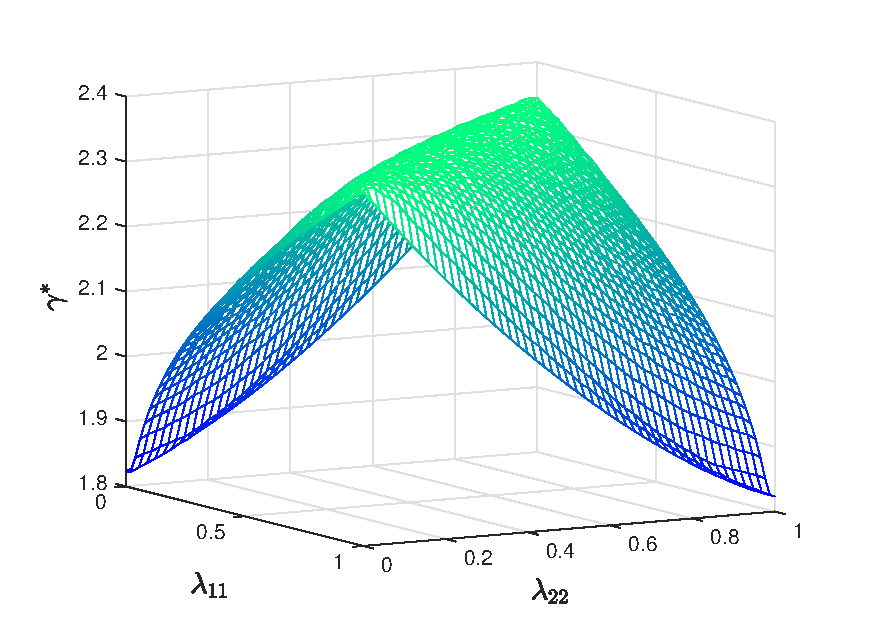
\includegraphics[scale=0.6]{./figures/lure_system/3d3.eps}\\ 
	\caption{最优 $l_2$性能增益 $\gamma^{*}$ 同条件模态转移矩阵 $\varPhi$的关系}
	\label{lure_fig1}
\end{figure}

首先,我们讨论一下最优$\ell_2$性能$\gamma^{*}$同模态转移概率$\varPhi$之间的关系。令
\begin{equation*}
\varPhi=\begin{bmatrix}
\lambda_{11}&1-\lambda_{11} \\
1-\lambda_{22}&\lambda_{22}
\end{bmatrix}
\end{equation*}
其中,$\lambda_{11},\lambda_{22} \in [0,1]$。 图\ref{lure_fig1} 表明最优 $l_2$性能增益 $\gamma^{*}$ 会随着 $\varPhi$的改变而改变。 同时可以观察到下面几个规律

	(1) 在 $\lambda_{11}=\alpha$, $\lambda_{22}=\beta$ 和 $\lambda_{11}=\beta$, $\lambda_{22}=\alpha$ 这两种情况下,$\gamma^{*}$的值是相同的。这个很好理解,毕竟模态的顺序是人为规定的,这两种情况只是将控制器模态定义的顺序改变了一下而已。
	
	(2) 在$\lambda_{11}=0$,$\lambda_{22}=0$ 或 $\lambda_{11}=1$, $\lambda_{22}=1$这两种情况时,最优$\ell_2$性能增益达到最小值 1.8236,实际上,根据我们之前的介绍,在这两种情况下,此时的控制器模态是同系统模态保持一致的,也就是说,这个时候的控制器是一个同步控制器。
	
	(3) 当$\lambda_{11}+\lambda_{22}$的值接近 1 的时候,	$\gamma^{*}$ 的值会变大,这是因为此时控制器的异步率提高了。


下面我们把条件模态转移矩阵中的参数设置为 $\lambda_{11}=0.4$, $\lambda_{22}=0.7$,来进一步研究系统的性能。可以得到如下控制器增益
\begin{equation}\notag
\begin{aligned}
K_{1}=\begin{bmatrix}
-1.4036&-1.3277
\end{bmatrix},\quad
\varGamma_{1}=-2.0473 \\
K_{2}=\begin{bmatrix}
-1.3908&-1.3080
\end{bmatrix},\quad
\varGamma_{2}=-1.8925
\end{aligned}
\end{equation}

\begin{figure}[!htb]
	\centering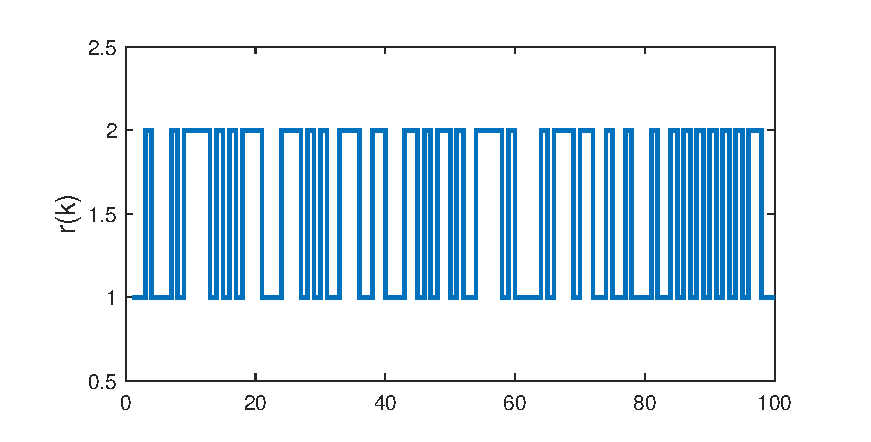
\includegraphics[scale=0.6]{./figures/lure_system/mode_p5.eps}\\ 
	\centering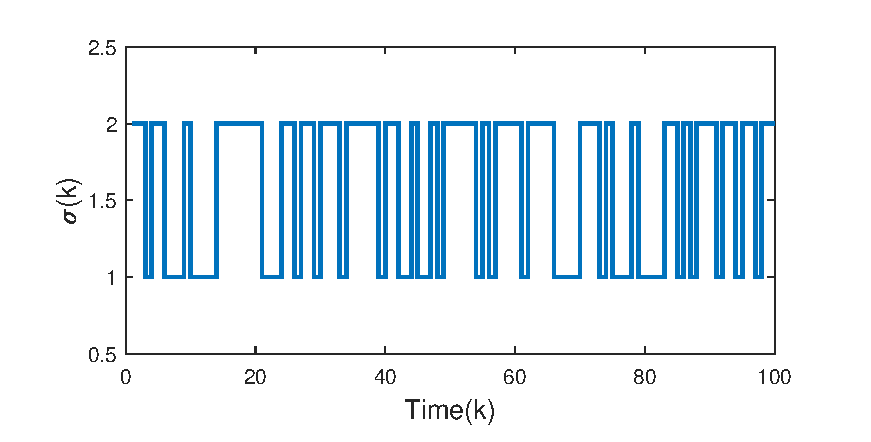
\includegraphics[scale=0.6]{./figures/lure_system/mode_k5.eps}\\ 
	\caption{系统及控制器模态}
	\label{lure_fig2}
\end{figure}

\begin{figure}[!htb]
	\centering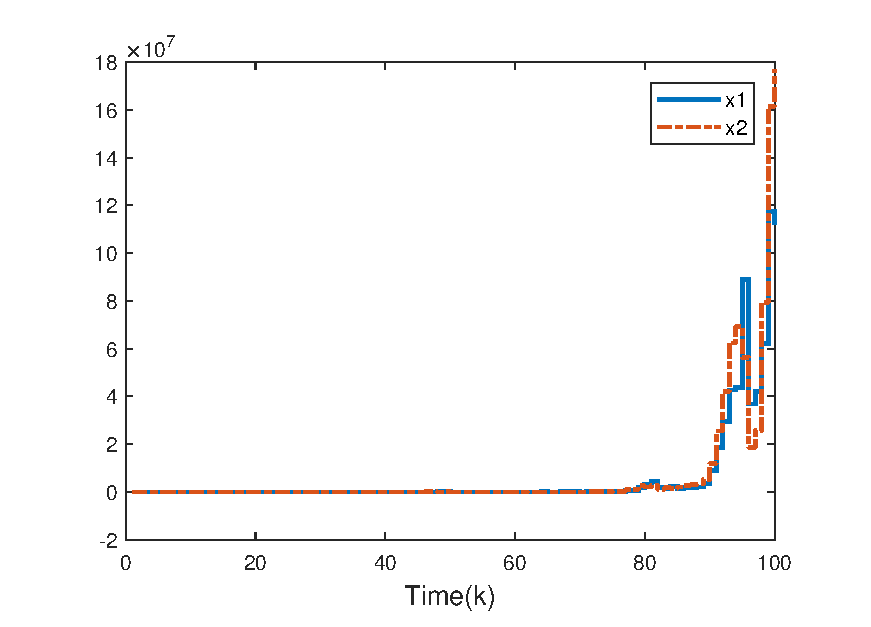
\includegraphics[scale=0.6]{./figures/lure_system/unstable_state2.eps}\\
	\caption{无控制率作用时系统状态变化}
	\label{lure_fig5}
\end{figure}

\begin{figure}[!htb]
	\centering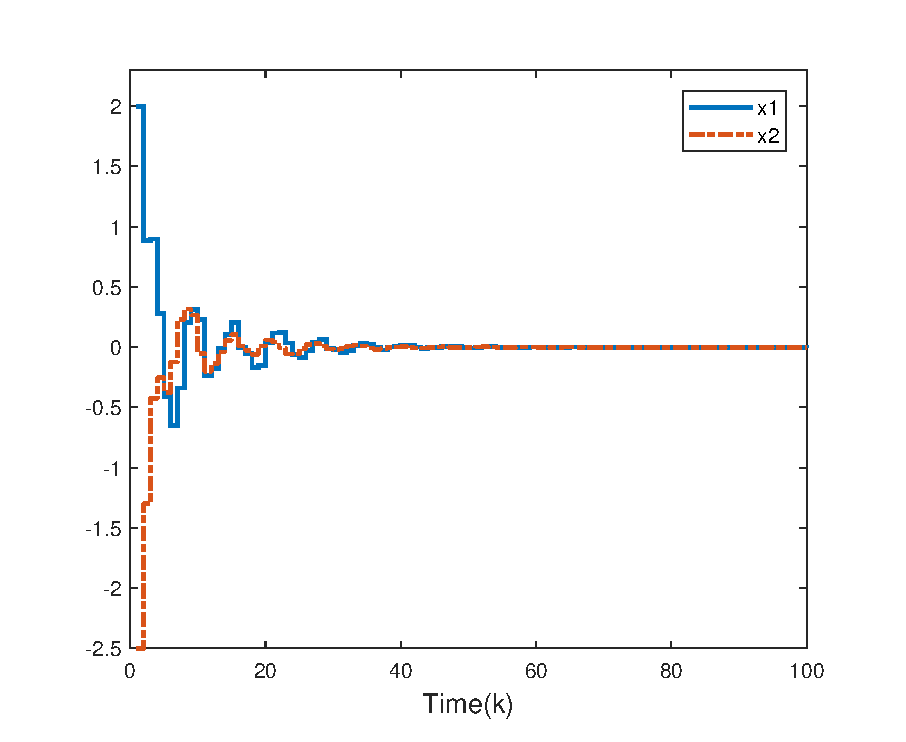
\includegraphics[scale=0.6]{./figures/lure_system/state4.eps}\\
	\caption{有控制率作用时系统状态变化}
	\label{lure_fig3}
\end{figure}
\begin{figure}[!htb]
	\centering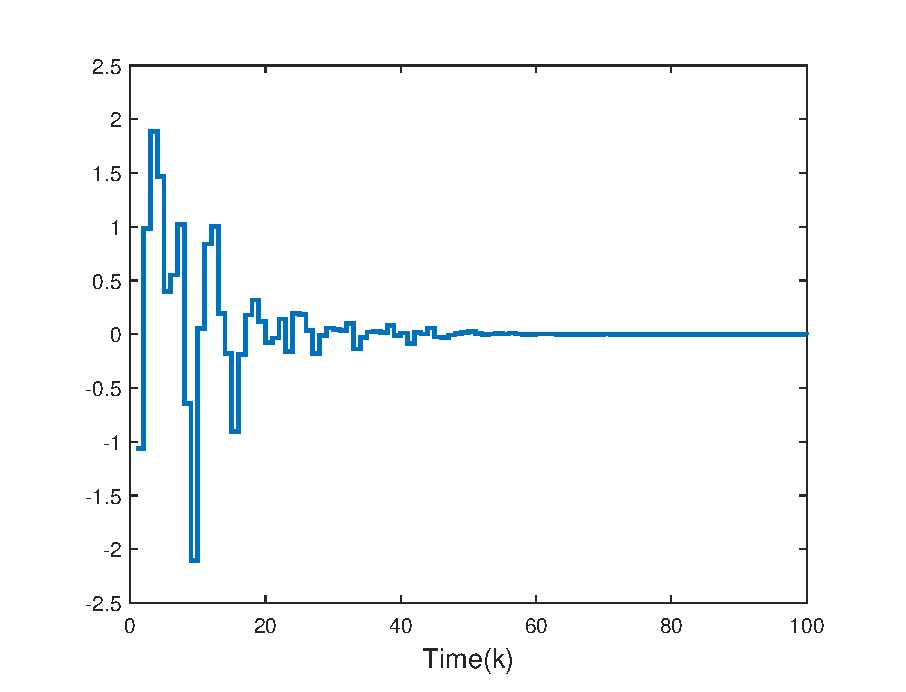
\includegraphics[scale=0.6]{./figures/lure_system/u_k3.eps}\\ 
	\caption{系统输入$u(k)$}
	\label{lure_fig4}
\end{figure}
图\ref{lure_fig2} 给出了一个控制器和系统模态的可能序列。此时,我们选择初始状态为 $x_{0}=\begin{bmatrix}
2&-2.5
\end{bmatrix}^{T}$,外部扰动设置为 $w_{k} = sin(k)*0.85^{k}$。 图\ref{lure_fig5} 表明,当系统在没有施加控制作用的时候是不稳定的。 当我们把控制率施加到系统上时,可以得到系统的状态轨迹如图\ref{lure_fig3}所示。同时,系统的输入$u_{k}$ 如图\ref{lure_fig4} 所示。 由图\ref{lure_fig3}、\ref{lure_fig4}, 我们可以看出,系统状态轨迹在施加我们设计的控制率以后会收敛,表明,此时系统是稳定的。上述实验表明,我们的控制器是异步的,且可以保证系统的稳定性,同时可以保证系统的$\ell_2$性能。


\section{小结}
	本章针对一类特殊的Markov跳变Lur'e系统,我们基于隐Markov模型,设计了一个异步控制器,使得待研究的系统在随机稳定的同时满足了一定的$\ell_2$性能。该异步控制器的特色在于,首先它是个异步控制器,因此比一般的同步控制器、模态独立控制器更加的灵活;其次,它由一个线行状态反馈和一个非线性输出反馈组成,对应了Lue'e系统的结构,这样的结构可以使得得到的结果更加不保守。 然后,根据得到的定理,提出了一个控制器的设计方法,进而设计的控制器可以使得满足系统随机稳定的同时得到最小的$\ell_2$性能。最后,我们通过了一个数值仿真例子验证了我们设计的控制器的有效性。